% 02.06.2016 12:00 CET last changed by a.holzinger
% General Template for LNCS and LNAI contributions based on llncs, adapted by ah
% Many thanks to the TRS team
% In case of using eps compile via 1) TeXify and then proceed with 2) dvi2pdf
%
\documentclass{llncs}
\usepackage{float}

\usepackage[dvips]{graphicx}
\usepackage[ruled,vlined]{algorithm2e}
\usepackage{amsfonts}
\usepackage{amssymb}
\usepackage{amsmath}
\usepackage{mathtools}

\providecommand{\abs}[1]{\lvert#1\rvert}
\providecommand{\norm}[1]{\lVert#1\rVert}

\usepackage{calc}
\usepackage{subfigure}

\usepackage{color}
\usepackage{soul}
\usepackage{comment}

\newtheorem{prop}{Property}

\newenvironment{Bitemize}{\renewcommand\labelitemi{\textbullet}\begin{itemize}}{\end{itemize}}

\begin{document}

\title{DO NOT DISTURB ? \\ Classifier behavior on perturbed datasets}

% \author{Bernd Malle\inst{1}\inst{2}, Peter Kieseberg\inst{1}\inst{2}, Edgar Weippl\inst{2}, Andreas Holzinger\inst{1}}

%\institute{Holzinger Group HCI-KDD \\
%Institute for Medical Informatics, Statistics \& Documentation\\
%            Medical University Graz, Austria\\
%            \texttt{b.malle@hci-kdd.org}
%\and
%SBA Research gGmbH, Favoritenstraße 16, 1040 Wien \\
%			\texttt{PKieseberg@sba-research.org}
%}
	
\maketitle

% ==================================
%				ABSTRACT
% ==================================
\begin{abstract}

Exponential trends in data generation are presenting today's organizations, economies and governments with challenges never encountered before, especially in the field of privacy and data security. One crucial trade-off regulators are facing regards the simultaneous need for publishing personal information for the sake of statistical analysis and Machine Learning in order to increase quality levels in areas like medical services, while at the same time protecting the identity of individuals. A key European measure will be the introduction of the General Data Protection Regulation (GDPR) in 2018, giving customers the 'right to be forgotten', i.e. having their data deleted on request. As this could lead to a competitive disadvantage for European companies, it is important to understand which effects deletion of significant data points has on the performance of ML techniques. In a previous paper we introduced a series of experiments applying different algorithms to a binary classification problem under anonymization as well as perturbation. In this paper we extend those experiments by multi-class classification and introduce outlier-removal as an additional scenario. While the results of our previous work were mostly in-line with our expectations, our current experiments revealed unexpected behavior over a range of different scenarios. A surprising conclusion of those experiments is the fact that classification on an anonymized dataset with outliers removed in beforehand can almost compete with classification on the original, un-anonymized dataset. This could soon lead to competitive Machine Learning pipelines on anonymized datasets for real-world usage in the marketplace.


\medskip

\textbf{Keywords}: Machine learning, knowledge bases, right to be forgotten, perturbation, k-anonymity, SaNGreeA, information loss, cost weighing vector, multi-class classification, outlier analysis, variance-sensitive analysis


\end{abstract}

\renewcommand{\thesubfigure}{\thefigure.\arabic{subfigure}}
\makeatletter
\renewcommand{\p@subfigure}{}
\renewcommand{\@thesubfigure}{\thesubfigure:\hskip\subfiglabelskip}
\makeatother


% ==================================
%			INTRODCUTION
% ==================================
\section{Introduction and Related Work}
\label{sect:introduction}

In today's data-driven industries which increasingly form the backbone of the 21st century's economy, personal information is no longer only stored by private companies, public service organizations or health providers. They also constitute a vital building-block for business intelligence and as a decision-making basis for improving services or public investments in measures for disease or natural disaster prevention. Therefore lies a crucial advantage in the publication, linkage, and systematic analysis of data sets from heterogeneous sources via statistics as well as Machine Learning. Any kind of institution which fails or is forbidden to engage in such activities, will in time face serious disadvantages on the marketplace or a lack in service quality compared to entities able to do so.

One specific challenge for data processing entities is increasingly imposed on them by the law. Under the new European General Data Protection Regulations (\textit{GDPR}) taking effect on June 1st, 2018, customers are given a \textit{right-to-be-forgotten}, meaning that an organization is obligated to remove a customer's personal data upon request. For many organizations, this would incur serious additional investments and costs from their IT infrastructure, as even backup- or statistical systems must be connected, lest no 'forgotten' data will reappear. Nevertheless, the law will allow data analysis on anonymized datasets (for which a right-to-be-forgotten makes no sense from a technical point of view), so that organizations will soon be faced with the question: Do we learn on original data \& bear all costs of the impeding bureaucracy, or shall we analyze anonymized datasets and risk significantly lower insights.

This brings us to the field of Privacy aware machine learning (PAML) \cite{DuchiJordan:2014:PrivacyAwareLearning}, enabled and fostered by concepts like \textit{k-anonymity} \cite{Samarati:2001:kAnonymity}, in which a record is released only if it is indistinguishable from at least $k-1$ other entities in the dataset. However, due to many personal records being high-dimensional in nature and k-anonymity being highly dependent on spatial locality (density) in order to effectively implement the technique in a statistically robust way, it might be difficult to anonymize data without suffering a high amount of information loss \cite{Aggarwal:2005:kAnonymity}.

Moreover, the original privacy requirement of \textit{k-anonymity} \cite{Sweeney:2002:k-Anonymity} has over time been refined by concepts like \textit{l-diversity} \cite{MachanavajjhalaEtAl:2007:l-Diversity} (in which every equivalence group must contain at least l diverse sensitive values from the original dataset), \textit{t-closeness} \cite{LiEtAl:2007:t-closeness} (which prescribes that the local distribution over sensitive values within an equivalence group must not differ from it's global distribution by more than a threshold $t$) as well as \textit{delta-presence} \cite{NergizClifton:2010:Delta-Presence} (which links the quality of anonymization to the risk posed by inadequate anonymization). Additionally, there is a whole discipline of measures summarized as \textit{differential privacy} \cite{dwork2008differential}, which deals with methods of securely releasing sensitive information upon database queries by injecting controlled noise into responses.

As far as PAML is concerned, a comparison of different Machine Learning algorithms on anonymized datasets was already conducted in 2014 \cite{Wimmer2014} by applying 6 different algorithms on 3 datasets, with very diverse results per algorithm. The main weakness of this paper is its usage of extremely differently-sized datasets which does not easily allow comparison; moreover they only used one very low privacy setting of $k=2$, preventing the authors from examining more interesting behavior as information content degrades further; this is a main point of our work.

The authors of \cite{Majeed2017} propose a scheme for controlling over-generalization of less identity-vulnerable QIs in diverse classes by determining the importance of QIs via Random Forest pre-computations as well as computing sensitive attribute diversity via the Simpson index \cite{simpson1949measurement}. Their resulting adaptive anonymization algorithm was compared to Mondrian \cite{lefevre2006mondrian} as well as IACk \cite{li2011information} and shows improvements w.r.t information loss as well as coverage (the number of descendant leaf nodes of generalized values in the taxonomy). Accuracy measured on classification tree, random forest and SVM shows equal or better performance when applied to a dataset anonymized by their proposed solution; it is interesting to note that their performance on large factors of $k$ not only remains stable, but in some cases increases with $k$, the same behavior we also observed in some of our experiments.

A recent paper \cite{LeeHCeiling2017} proposes the introduction of an additional requirement for anonymization on top of k-anonymity called h-ceiling, which simply restricts generalizations within an equivalence class to a certain level below suppression. In the case on an equivalence class being able to satisfy h-ceiling but not k-anonymity (their method applies full-domain generalization), counterfeit records are inserted into the respective group; each insertion is also collected in a journal which is eventually published with the anonymized data. Their approach unsurprisingly yields lower reconstruction error and information loss as well as more fine-grained query results due to less generalization. However, their experiments mostly fix $k=5$ and therefore simply try to reduce information loss due to anonymization, but do not try to examine ML performance over a wider range of k factors; moreover, there seems to be some inconsistency in their predictions.

Finally, we should also reference our previous work on this topic \cite{malle2016right}, in which we conducted a comparison study of binary classification performance on perturbed (selective deletion) vs. wholesale anonymized data. Our experiments showed that perturbation was still significantly less damaging to Machine Learning performance than even slight anonymization; that state of our previous research marks the connecting point to this paper.



% ==================================
%		BASICS OF K-ANONYMITY
% ==================================
\section{K-Anonymity and Information loss}

While there are several data-structures which can contain and convey personal information we might want to protect (free text, audio, images, graph structures etc.) we are focusing our work on tabular data, since most unstructured documents of sensitive nature today can be mapped to tabular data and since delicate information is most easily extracted from those. Figure~\ref{fig:anon_categories} illustrates the original tabular concept of three different categories of data we will encounter in such tables:

\begin{itemize}
	\item \textbf{Identifiers} directly reveal the identity of a person without having further analysis of the data. Examples are first and last names, email address or social security number (SSN). As personal identifiers are hard to generalized (see Figure~\ref{fig:gen_hierarchy}) in a meaningful way (truncating an email address to 'host' would not yield much usable information), those columns are usually removed. The figure displays this column in a red background color.
	\item \textbf{Sensitive data,} or 'payload', is crucial information for statisticians or researchers and can therefore not be erased or perturbed; such data usually remains untarnished within the released dataset. The table shows one column in green background color representing such data.
	\item \textbf{Quasi identifiers (QI's)}, colored in the table with an orange background, do not directly identify a person (age=35), but can be used in combination to restrict possibilities to such a degree that a specific identity follows logically. For instance, \cite{sweeney2002k} mentioned that 87\% of U.S. citizens in 2002 could be re-identified by just using the 3 attributes \textit{zip code}, \textit{gender} and \textit{date of birth}. On the other hand, this information might hold significant information for the purpose of research (e.g. zip code could be of high value in a study on disease spread). Therefore we generalize this kind of information, which means to lower its level of granularity. As an example, one could generalize grades from A+ to B- into A's and B's and then further up to encompass 'all' (also denoted as '*'), as shown in Figure~\ref{fig:gen_hierarchy}.
\end{itemize}

\begin{figure}[H]
	\begin{center}
		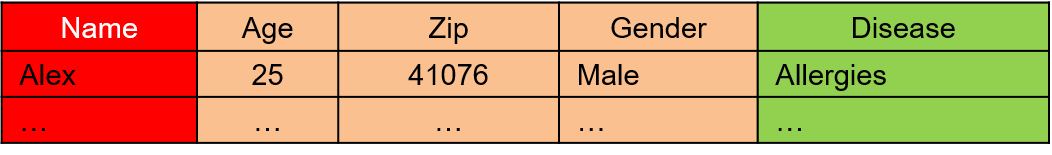
\includegraphics[width=0.9\textwidth]{figures/theory/3typesofdata}
		\caption{The three types of data considered in (k-)anonymization}
		\label{fig:anon_categories}
	\end{center}
\end{figure}

As described in \cite{ciriani2007kappa}, k-anonymization requires a data release to contain at least $k-1$ duplicate entries for every occurring combination of attributes. One can imagine this as a clustering problem with each cluster's (also called \textit{equivalence class}) quasi-identifier state being identical for every data point it contains. One can achieve this via suppression and generalization, where by suppression we mean simple deletion, whereas generalization refers to a decrease in a value's granularity. As an example, in Figure~\ref{fig:anonymized_clusters}, an input dataset has been transformed through k-anonymization into a clustered set with each cluster being at least of $size = 3$; thus the data is said to be $3-anonymized$.

\begin{figure}[h]
	\centering
	\begin{minipage}[b]{0.535\textwidth}
		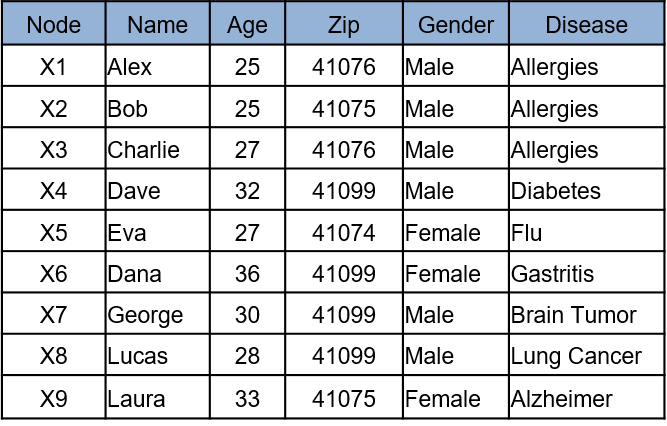
\includegraphics[width=\textwidth]{figures/theory/k_anon_input}
	\end{minipage}
	\hfill
	\begin{minipage}[b]{0.448\textwidth}
		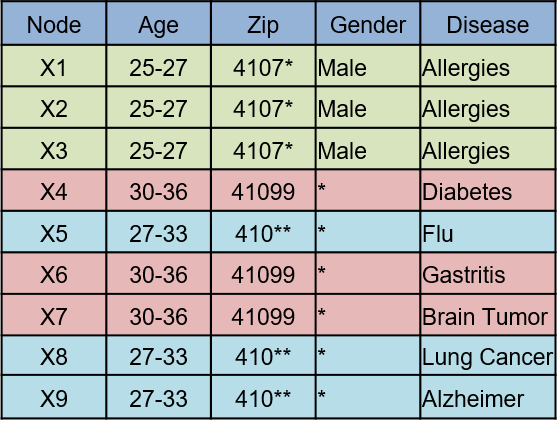
\includegraphics[width=\textwidth]{figures/theory/k_anon_output}
	\end{minipage}
	\caption{Tabular anonymization: input table and anonymization result}
	\label{fig:anonymized_clusters}
\end{figure}

Generalization works through a concept called \textit{generalization hierarchies / taxonomies}, which run from leaf nodes denoting particular values ('France') via internal nodes ('Western Europe') to their most general root ('all countries' or '*'). Such a hierarchy is depicted in Figure~\ref{fig:gen_hierarchy}. In generalizing the original input value, one traverses the tree from a leaf node upwards until a certain condition is met. In the case of k-anonymity, we satisfy this condition when we can construct an equivalence group with all quasi-identifiers being duplicates of one another.

\begin{figure}[h]
	\begin{center}
		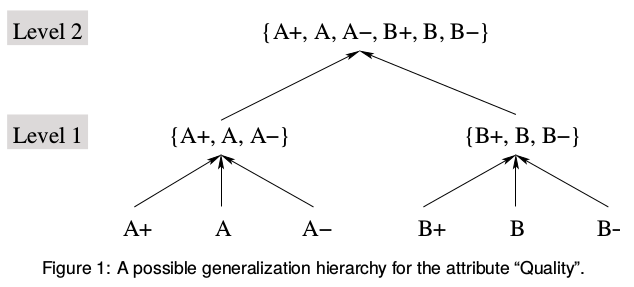
\includegraphics[width=0.8\textwidth]{figures/theory/gen_hierarchy}
		\caption{Example of a typical generalization hierarchy}
		\label{fig:gen_hierarchy}
		\small
		taken from \cite{aggarwal2005approximation}
	\end{center}
\end{figure}


As each level of generalization invokes an increasing loss of specificity, we do not want to construct our clusters inefficiently, but minimize a dataset's overall information loss \cite{aggarwal2005approximation}. This makes k-anonymization an NP-hard problem due to an exponential number of possible data-row combinations one can examine.



% ==================================
%				EXPERIMENTS
% ==================================
\section{Experiments}
\label{sect:experiments}

The following sections will describe our series of experiments in detail, encompassing the dataset used, the algorithms chosen for classification as well as a description of the overall process employed to obtain our results.


\subsection{Data} 
\label{ssect:data}

As input data we chose the training set of the adults dataset from the UCI Machine Learning repository which was generated from US census data and contains approximately 32,000 entries (30162 after deleting rows with incomplete information). All but one columns were considered for experimentation, the remaining representing duplicate information (education $=>$ education\_num). Figure~\ref{fig:adult_original_distribution} shows the attribute value distribution of 6 arbitrarily selected columns of the original (un-anonymized) dataset.


\begin{figure}[!h]
	\begin{center}
    \hspace*{-0.8cm}
		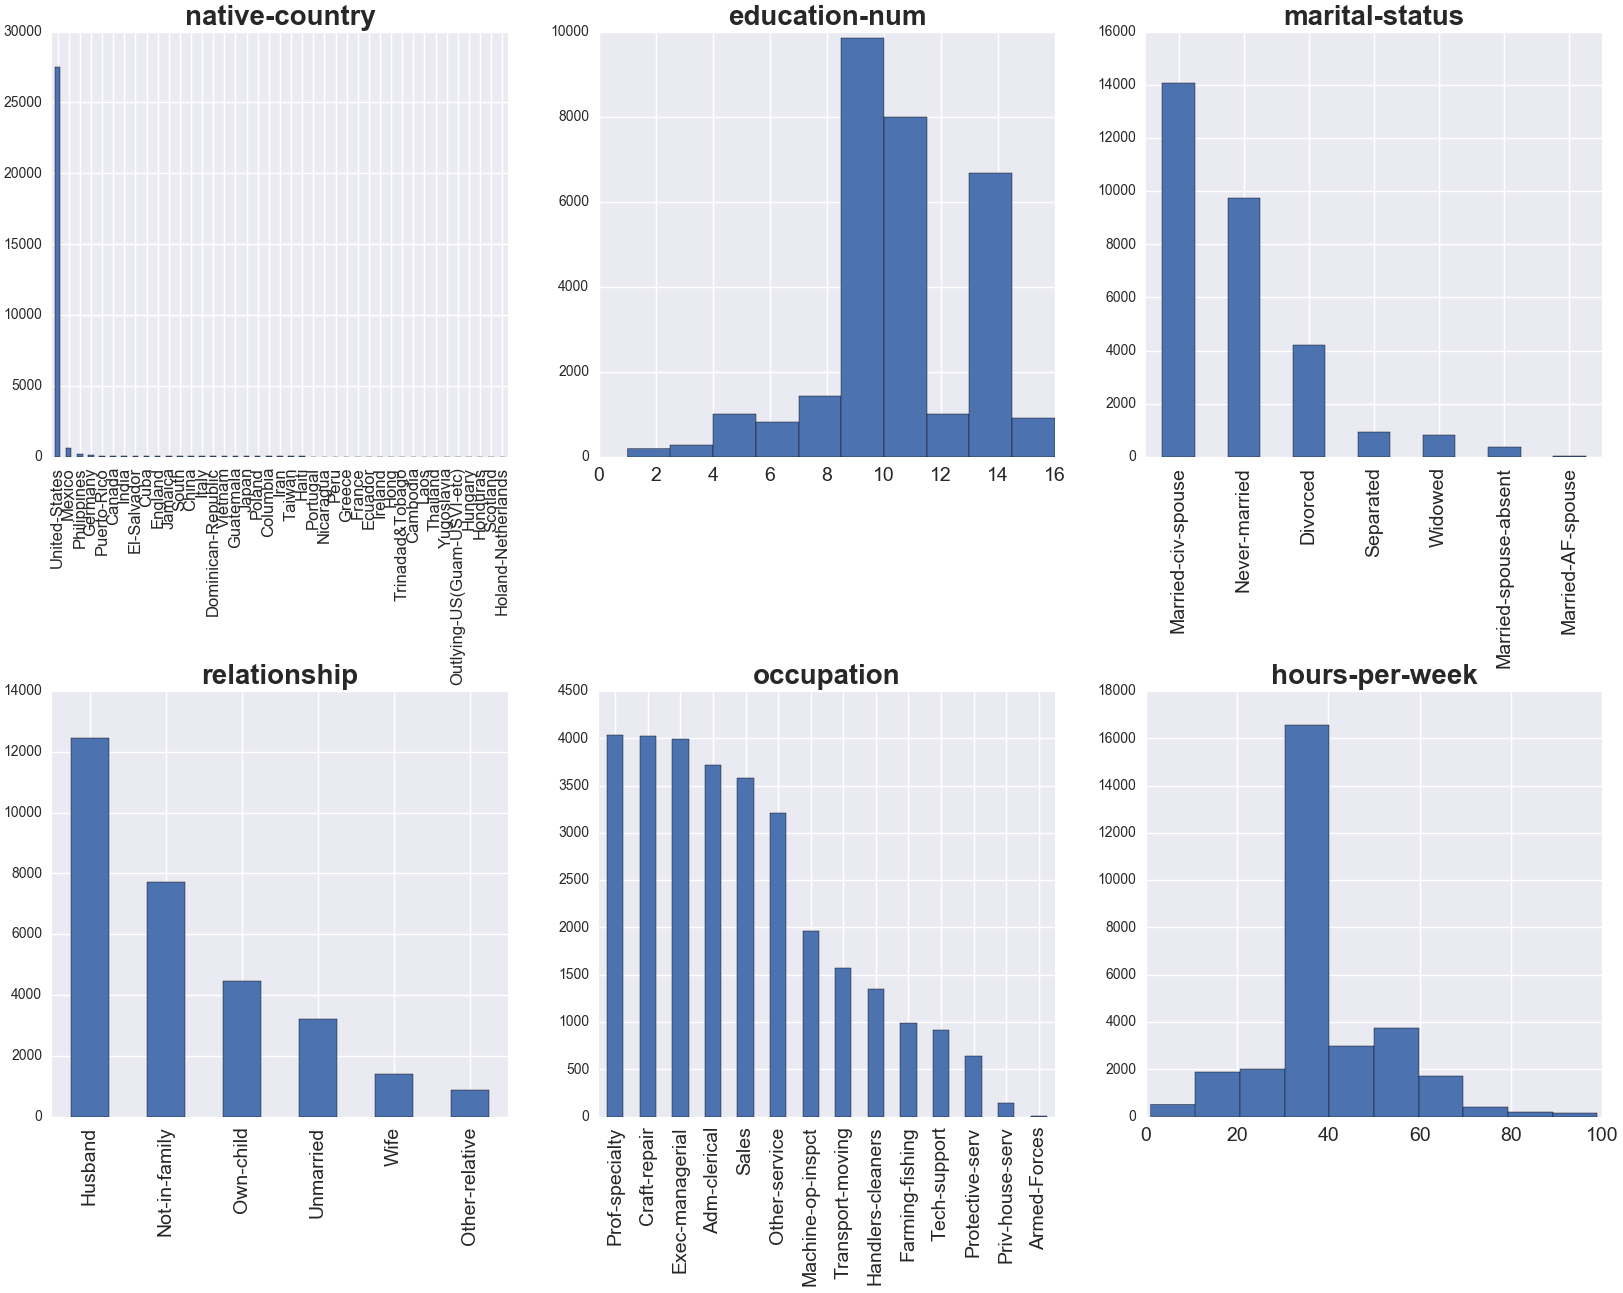
\includegraphics[width=1.1\textwidth]{figures/theory/dist_initial_small}
		\caption{Initial distribution of six selected data columns of the adult dataset.}
		\label{fig:adult_original_distribution}
	\end{center}
\end{figure}

Amongst these distribution, two clearly stand out: \textit{native-country} as well as \textit{hours-per-week}, which are both dominated by a single attribute value (\textit{United-States} and \textit{40}, respectively). In order to demonstrate the effect of anonymization on attribute value distributions, Figure~\ref{fig:adult_anonymized_distribution} shows the same attribute distributions under anonymization by a factor of $k=19$. Although the dominance of the \textit{United-States} was successfully "broken" by this method, in several instances the \textit{generalized-to-all}-value (*) now skews the data set even more. In addition to the incurred information loss this might be another reason for degraded classifier performance on such data.

\begin{figure}[!h]
	\begin{center}
    	\hspace*{-0.8cm}
		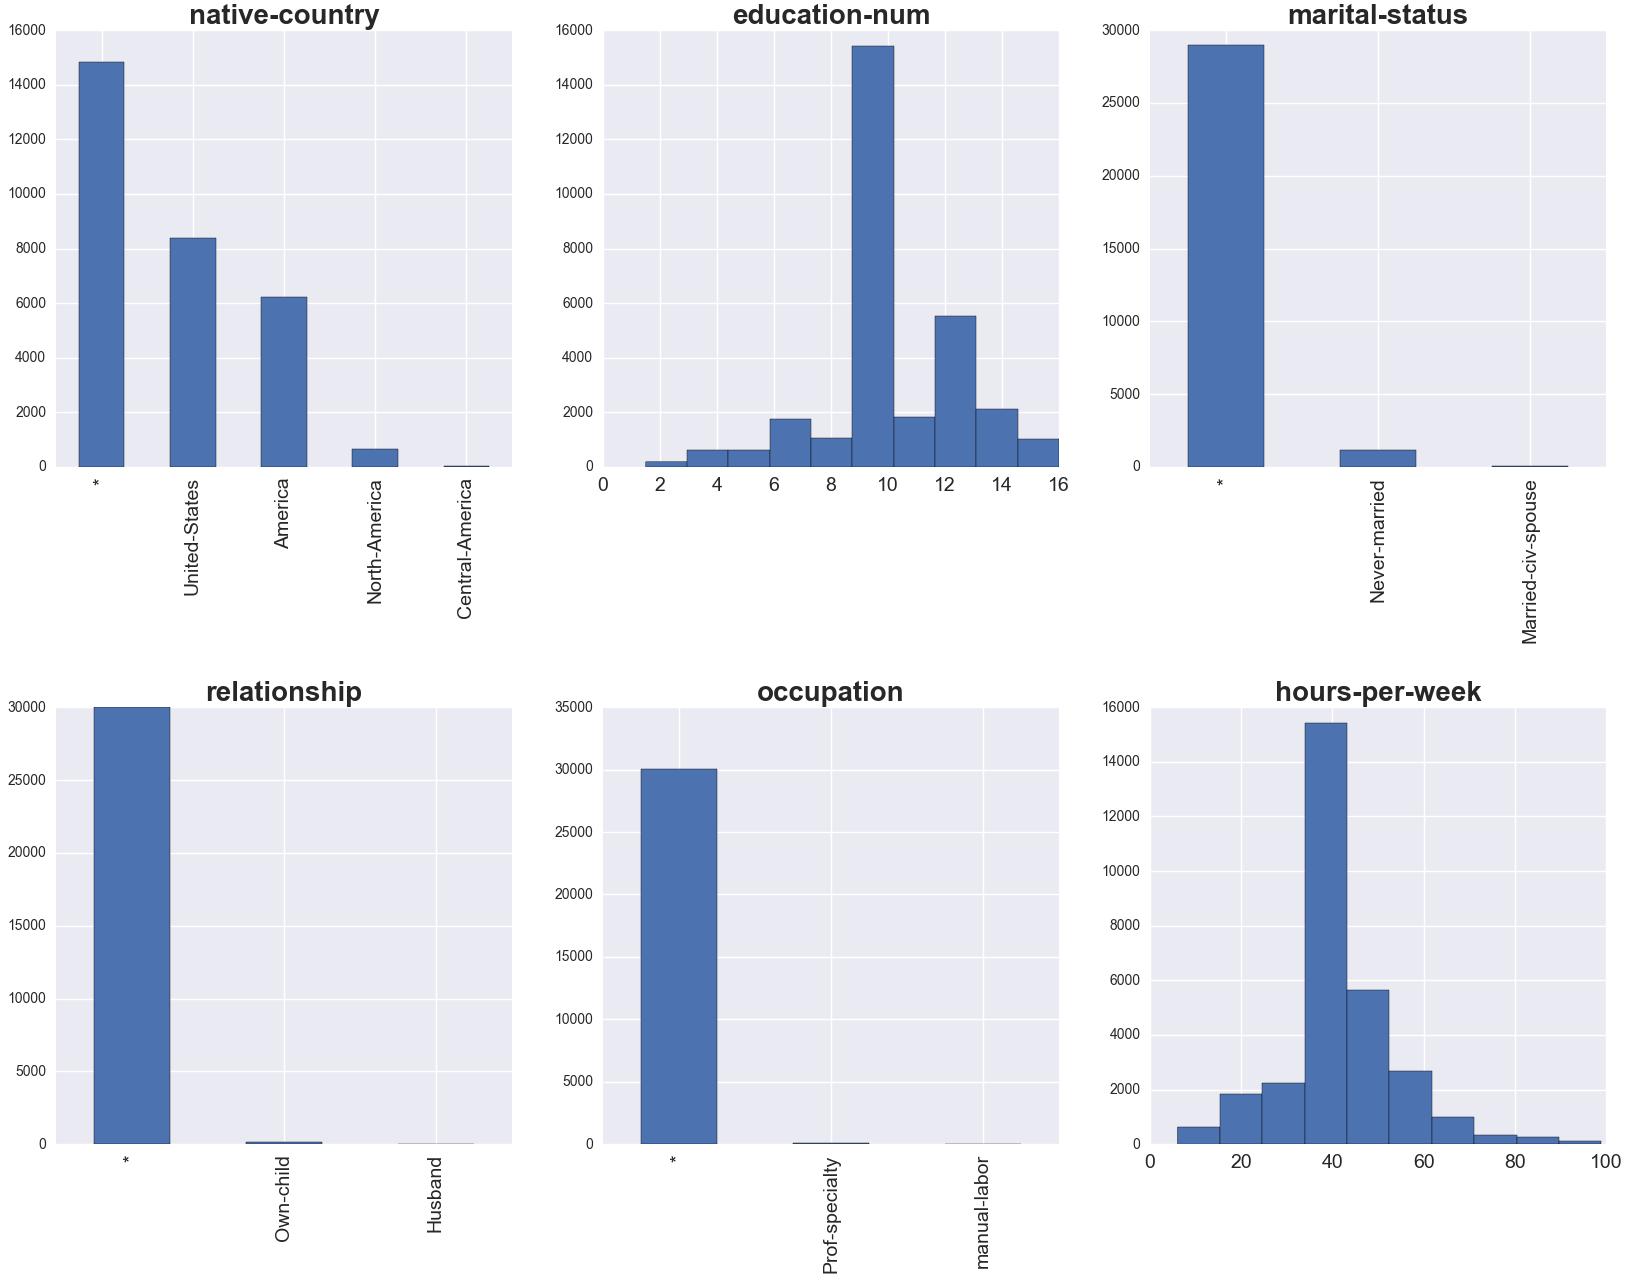
\includegraphics[width=1.1\textwidth]{figures/theory/dist_anonym_small}
		\caption{Anonymized distribution of six selected data columns of the adult dataset, anonymization factor $k=19$, with equal weight for each attribute.}
		\label{fig:adult_anonymized_distribution}
	\end{center}
\end{figure}



\subsection{Anonymization Algorithm}
\label{ssect:algorithm}

We implemented our own version of a greedy clustering algorithm called SaNGreeA (Social network greedy clustering, \cite{campan2009data}) in JavaScript mainly for three reasons: 1) apart from 'normal' tabular anonymization tt has a network anonymization component based on stochastic reconstruction error, so it is possible for us to use this algorithm in later works regarding the impact of anonymization on graph algorithms; 2) we wanted a simple conceptual model so we could interact with the algorithm and thus conduct interactive Machine Learning experiments in the future (those experiments are well under way at the time of this writing); 3) we wanted an algorithm capable of running in the browser so we could run our experiments online especially w.r.t. 2). The main downside of this choice is the reduced algorithmic performance of $O(n^2)$ as well as a further slow-down for JS vs native code of a factor of about $3-4$. In the future, we will strive to implement faster algorithms which nevertheless retain properties suitable for our needs, narrowing down the simplicity - performance trade-off.

As mentioned, SaNGreeA consists of two strategies for tabular as well as network anonymization, with two respective metrics for information loss. The \textit{Generalization Information Loss} or \emph{GIL} consists of a categorical as well as a continuous part, with the former measuring the distance of a level-of-generalization from it's original leaf node in the generalization hierarchy (taxonomy), while the latter measures the range of a continuous-valued generalization (e.g. age cohort [35-40]) divided by the whole range of the respective attribute (e.g. overall age-range [17-90]).


\begin{equation*}
\begin{split}
\text{GIL}(cl) = \abs{cl} \cdot (\sum_{j=1}^{s} \frac{size(gen(cl)[N_j])}{size(min_{x \epsilon N} (X[N_j]), max_{x \epsilon N} (X[N_j]))} \\ 
+ \sum_{j=1}^{t} \frac{height(\Lambda(gen(cl)[C_j]))}{height(H_{C_j})})    
\end{split}
\end{equation*}


where:\\
- $\abs{cl}$ denotes the cluster cl's cardinality; \\
- $size([i1,i2])$ is the size of the interval $[i1,i2]$, i.e., $(i2-i1)$; \\
- $\Lambda(w), w \epsilon H_{C_j}$ is the sub-hierarchy of $H_{C_j}$ rooted in $w$; \\
- $height(H_{C_j})$ denotes the height of the tree hierarchy $H_{C_j}$; \\


The total generalization information loss is then given by:

\begin{equation*}
\text{GIL}(G,S) = \sum_{j=1}^{v} \text{GIL}(cl_j)
\end{equation*}
And the normalized generalization information loss by:
\begin{equation*}
\text{NGIL}(G,S) = \frac{\text{GIL}(G,S)}{n \cdot (s+t)}
\end{equation*}


As for the networking-part of this algorithm, it introduces a measure called \textit{structural information loss} (SIL). The SIL is composed of two different components, which represent statistical errors of 1) intra-cluster as well as 2) inter-cluster reconstruction.

For the exact mathematical definitions of SIL \& NSIL the reader is kindly referred to the original paper. Because the structural information loss cannot be computed exactly before the assembly of all clusters is completed, the exact computations were replaced by the following distance measures: \\

Distance between two nodes:
\begin{equation*}
\text{dist}(X^i, X^j) = \frac{\abs{\{l|l=1..n \wedge l \ne i,j;b_l^i \ne b_l^j}}{n-2}
\end{equation*}

Distance between a node and a cluster:
\begin{equation*}
\text{dist}(X, cl) = \frac{\sum_{X^j \epsilon cl} \text{dist}(X, X^j) }{\abs{cl}}
\end{equation*}

Since SaNGreeA follows the greedy-clustering paradigm, it runs in quadratic time w.r.t. the input size in number of nodes. This worked well within milliseconds for a problem size of a few hundred nodes, but took up to 60 minutes on the whole adult training dataset. Finally, as stated above, we chose SaNGreeA for its intuitive simplicity and graph anonymization capabilities, the latter of which are serving us well in a different branch of our ongoing research efforts; for the experiments in this paper, we restricted ourselves to the tabular anonymization capabilities of the algorithm.


\subsection{Dataset creation}
\label{ssect:dataset_creation}

To examine the effect of perturbation, anonymization, outlier-removal as well as outlier-removal+anonymization on classifier performance, we designed the following processing pipeline:


\begin{enumerate}
	\item Taking the original (preprocessed) dataset as input, we transformed its attributes to boolean values, so instead of \textit{native-country $->$ United-States} we considered \textit{United-States $->$ yes / no}.
	\item We ran 4 different classifiers on the resulting data and computed their respective F1 score. The 4 classifiers used were \textit{gradient boosting} representing the boosting paradigm, \textit{random forest} representing the bagging technique, \textit{logistic regression} as a representative of categorical prediction via optimization of a coefficient vector, as well as \textit{linear SVC} representing Support Vector Machines constructing hyperplanes in sufficiently high-dimensional spaces.
	\item For our perturbation experiments, we extracted the most / least significant attribute values according to the logit coefficients as depicted in Figure~\ref{fig:adult_important_columns}. For each of these attribute values, we subsequently deleted a specific percentage $p \in \{0.2, 0.4, 0.6, 0.8, 1.0 \}]$ of data rows containing that value, resulting in a series of new datasets of reduced size.
	\item In order to measure the effects of k-anonymization on classifier performance, we applied SaNGreeA's GIL component to generate datasets with a k-factor of $k \in \{3, 7, 11, 15, 19, 23, 27, 31, 35, 100\}$. Furthermore, we used each of these settings with 3 different weight vectors: 1) equal weights for all attributes, 2) age information preferred ($\omega(age)=0.88$, $\omega(other\_attributes)=0.01$) and 3) race information preferred ($\omega(race)=0.88$, $\omega(other\_attributes)=0.01$).
	\item The outlier-removal datasets were created by executing scikit-learn's Isolation-Forest in order to identify and remove outliers in a range of $5\% - 95\%$ (stepsize: $5\%$) from the original dataset. This resulted in 18 new datasets for analysis.
	\item Finally, in order to analyze classifier performance on an outlier/anonymization combination, we repeated the procedure described for anonymization on a surrogate dataset that had $30\%$ of its outliers removed in beforehand.
\end{enumerate}


\begin{figure}[!h]
	\begin{center}
		% \vspace{-1.0cm}
    	\hspace*{-0.8cm}
		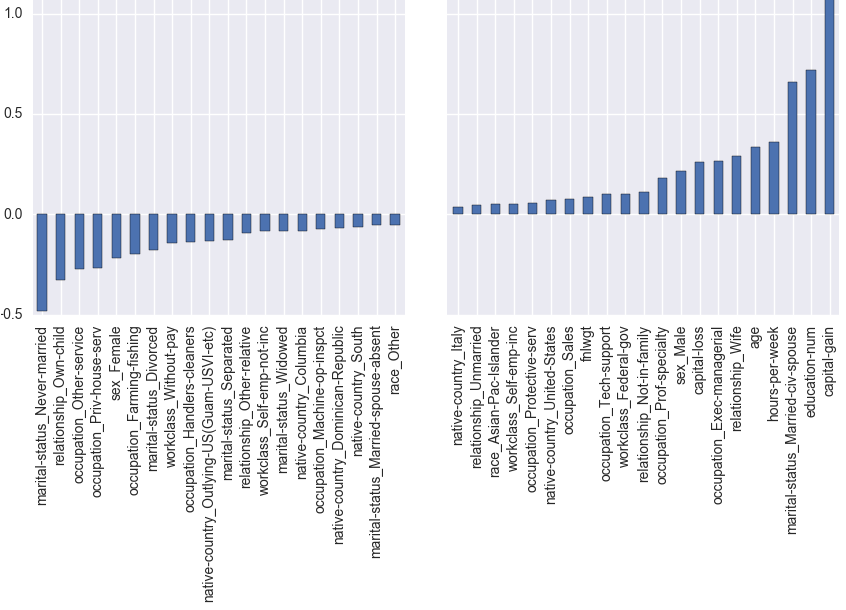
\includegraphics[width=1.1\textwidth]{figures/theory/important_columns_income_truncated}
		\caption{Attribute values within the adult dataset which contribute highest / lowest certainty to the classification of income (truncated at ~1.0). The rightmost columns represent information which enable a classifier to discern most clearly between classes, while the leftmost columns (depending on their actual score) could even confuse the algorithm. We chose this example because income is a binary decision, so the values don't change per category to predict.}
		\label{fig:adult_important_columns}
	\end{center}
\end{figure}



% ==================================
%		RESULTS & DISCUSSION
% ==================================
\section{Results \& Discussion}
\label{sect:results}


\subsection{Perturbed Datasets - Selective Deletion}
\label{ssect:selective_deletion}

In order to be able to compare the impact of selectively deleting the most / least important attribute values (in fact, the whole data points containing those values) on different classifiers, we chose to select these values via examining the logit coefficients produced during logistic regression. Although this possibly entails non-erasure of the values specifically significant for each classifier, we chose algorithmic comparison as the more insightful criterion; the implicit assumption that the same attribute values would influence all classifiers approximately equally was largely confirmed by our results.

In contrast to binary classification, determining the 'right' values to delete for a multi-class problem is not always possible: Values contributing highly to the decision boundary for one class might be less significant in the case of another - accordingly one would expect inconclusive behavior in the case of a target for which the highest / lowest log coefficients do not line up over class boundaries.

For each of the targets 'marital-status' and 'education-num' we measured those interesting coefficients in the hope of improving / degrading algorithmic performance; that means deletion of highest logit's is supposed to remove certainty from an algorithm and decreasing performance, while deletion of lowest logit's is supposed to remove uncertainty, thus improving performance. Our analysis showed that while 'marital-status' had mainly the same most / least significant logit's across all classes, the attribute values for 'education-num' were rather diverse in this area.

In the latter case this lead to erratic behavior of the resulting performance curves, as can be seen in (Figure~\ref{fig:results_perturbation_education_num}). It is interesting to note that 'income$\_>$50k' obviously held much larger significance for Logistic Regression than for the other classifiers, as their results showed f1 score improvement with this particular value eviscerating.


\begin{figure}[!h]
	\centering
	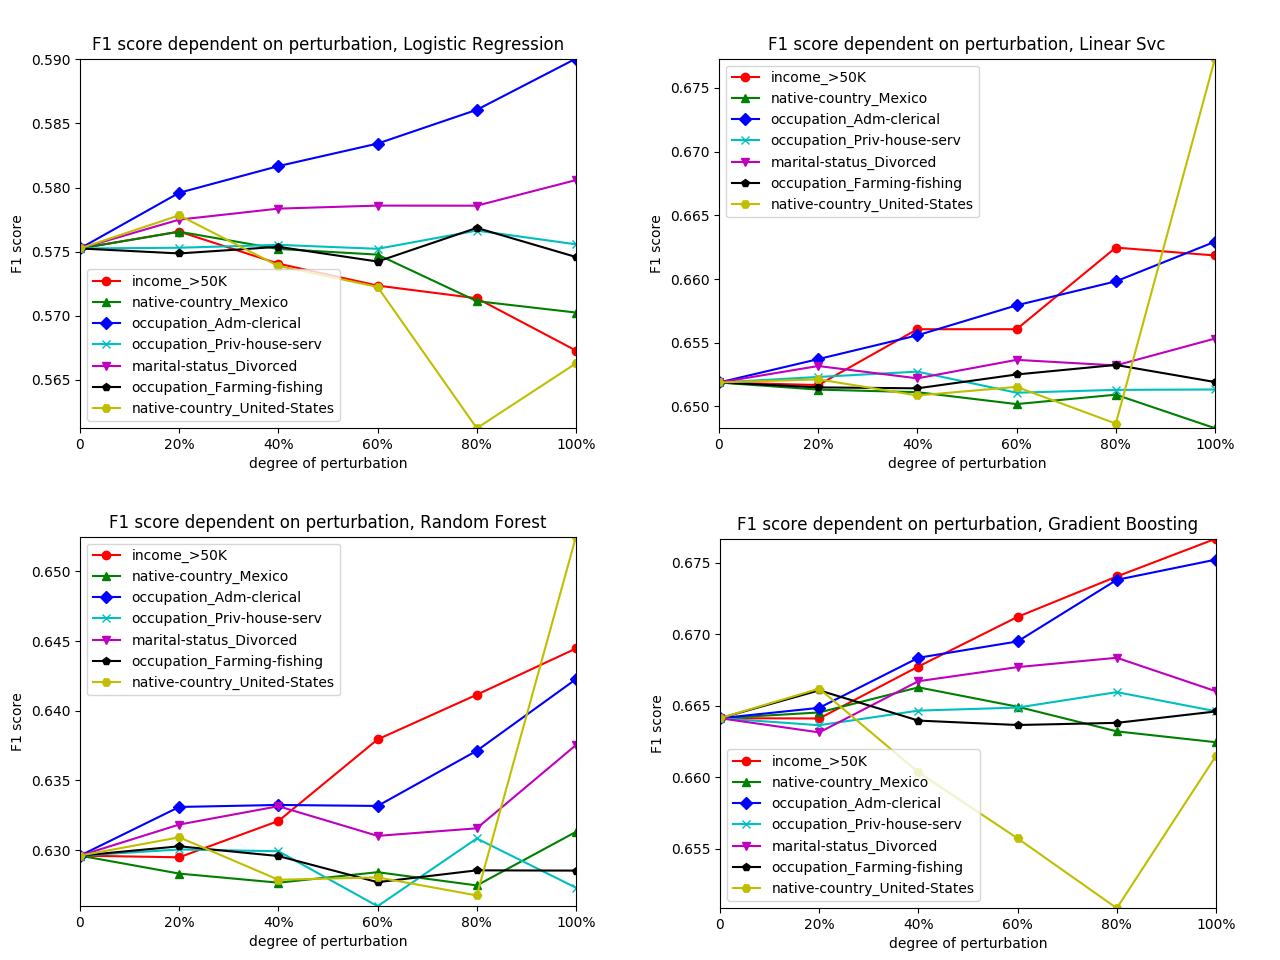
\includegraphics[width=1\textwidth]{figures/perturbation/adults_education_num/perturb_education_combined}
	\caption{Multi-class classification on target \textit{education-num} under perturbation by selective deletion of the most / least contributing attribute values. Since different values are significant for deciding on different classes of education level, progressive deletion of this data results in indeterminate behavior.}
	\label{fig:results_perturbation_education_num}
\end{figure}


In the case of 'marital-status' almost the same attribute values were rated as most / least significant across all classes - this results in very clear outputs with the erasure of highly important values decreasing performance drastically while deletion of confusing values leading to a significant increase in classifier performance (Figure~\ref{fig:results_perturbation_marital_status}). While it is not surprising that relationship information shows high correlation with marital status, the opposite effects of \textit{sex\_Female} and \textit{sex\_Male} stand out as a slight curiosity - being a woman in this dataset seems to point less distinctly to a specific marital status than being a man.


\begin{figure}[!h]
	\centering
	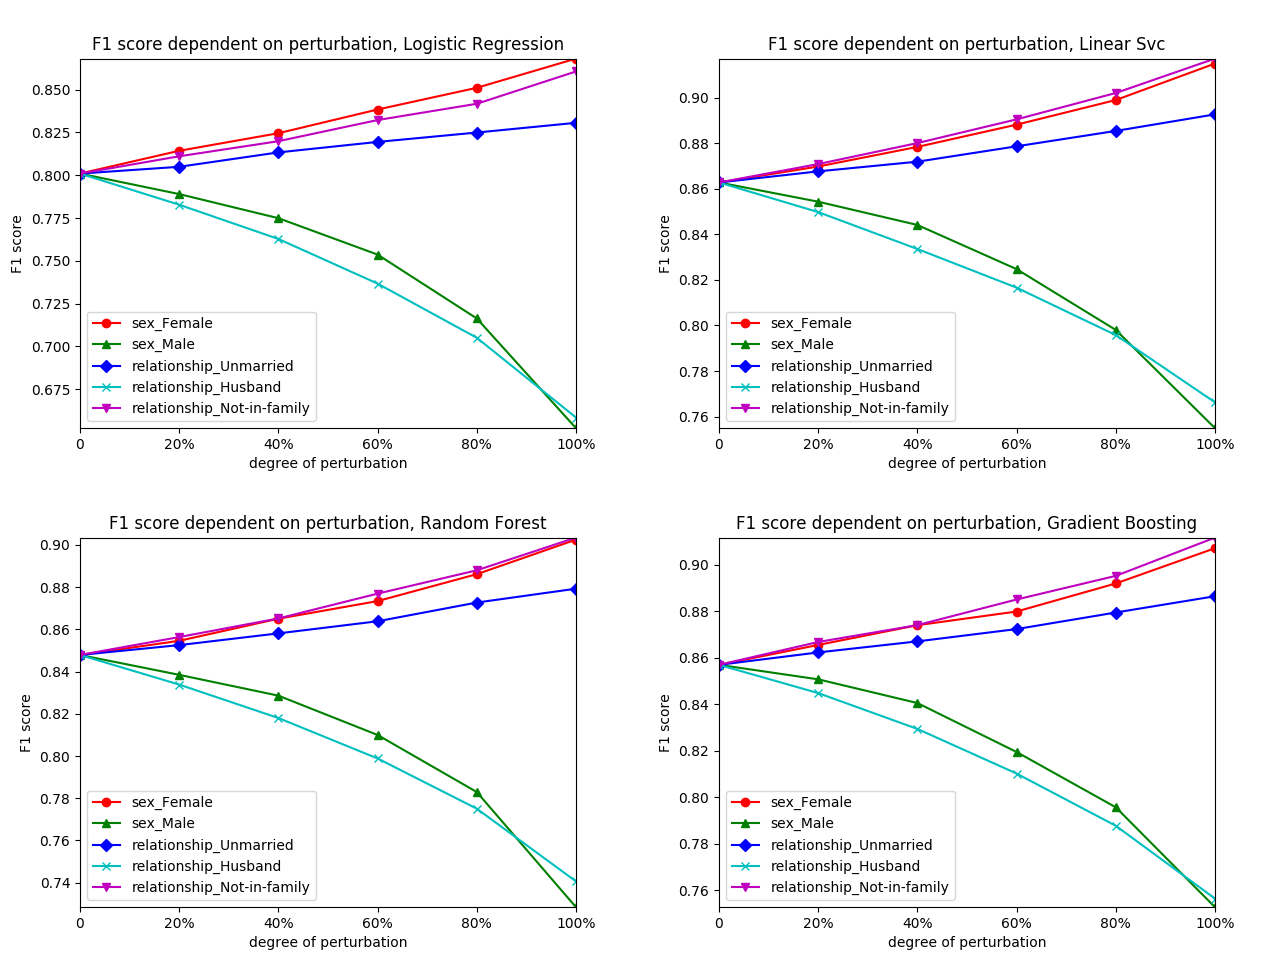
\includegraphics[width=1\textwidth]{figures/perturbation/adults_marital_status/perturb_marital_combined}
	\caption{Multi-class classification on target \textit{marital-status} under perturbation by selective deletion of the most / least contributing attribute values. Since the same values are significant for deciding different classes of marital status, progressive deletion leads to orderly increase / decrease of ML performance.}
	\label{fig:results_perturbation_marital_status}
\end{figure}



\subsection{Anonymized Datasets}
\label{ssect:anonymized_ds}

Analogous to our previous work \cite{malle2016right} we performed anonymization on the adult dataset for a range of values of $k$, but this time extending the range to $k \in \{3, 7, 11, 15, 19, 23, 27, 31, 35, 100\}$ for a broader observational basis of algorithmic behavior, especially towards higher values of $k$, as already conducted by other researchers \cite{Majeed2017}, \cite{LeeHCeiling2017}. As we set out to examine multi-class classification performance, we chose the 'marital-status' and 'education-num' columns of the adult dataset as targets, treating income as an independent input feature. For 'marital-status' we left the 7 categorical values in the original dataset unchanged, whereas we clustered the 16 continuous 'education-num' levels into the 4 groups 'elementary school', 'high school including graduate', 'college up to Bachelors' as well as 'advanced studies'.

Our observation generally show the same type of behavior than in our previous experiments on target \textit{income}, with one notable exception: The Random Forest classifier shows a sharp drop in algorithmic performance when operating on the very skewed 'age' and 'race' feature vectors, only to recover its discriminative power and increase in performance up to a $k$ of $100$. We also note a somewhat similar behavior for Logistic Regression, albeit not as distinctly. A possible explanation for this behavior could lie in the \textit{bagging}-nature of Random Forest, meaning that the algorithm bootstraps by randomly sampling data-points from the overall population into possibly overlapping bags of 'local' data. As larger swaths of the input data become more and more equal with increasing levels of $k$, this would lead to less local over-fitting, thus making the job easier for a global averaging-strategy to filter out variance and improve generalization ability. However, if this was true, the maximum performance should not be recorded on the original (un-anonymized) dataset, thus we are currently at a loss of an adequate explanation for this specific case.


\begin{figure}[!h]
	\centering
	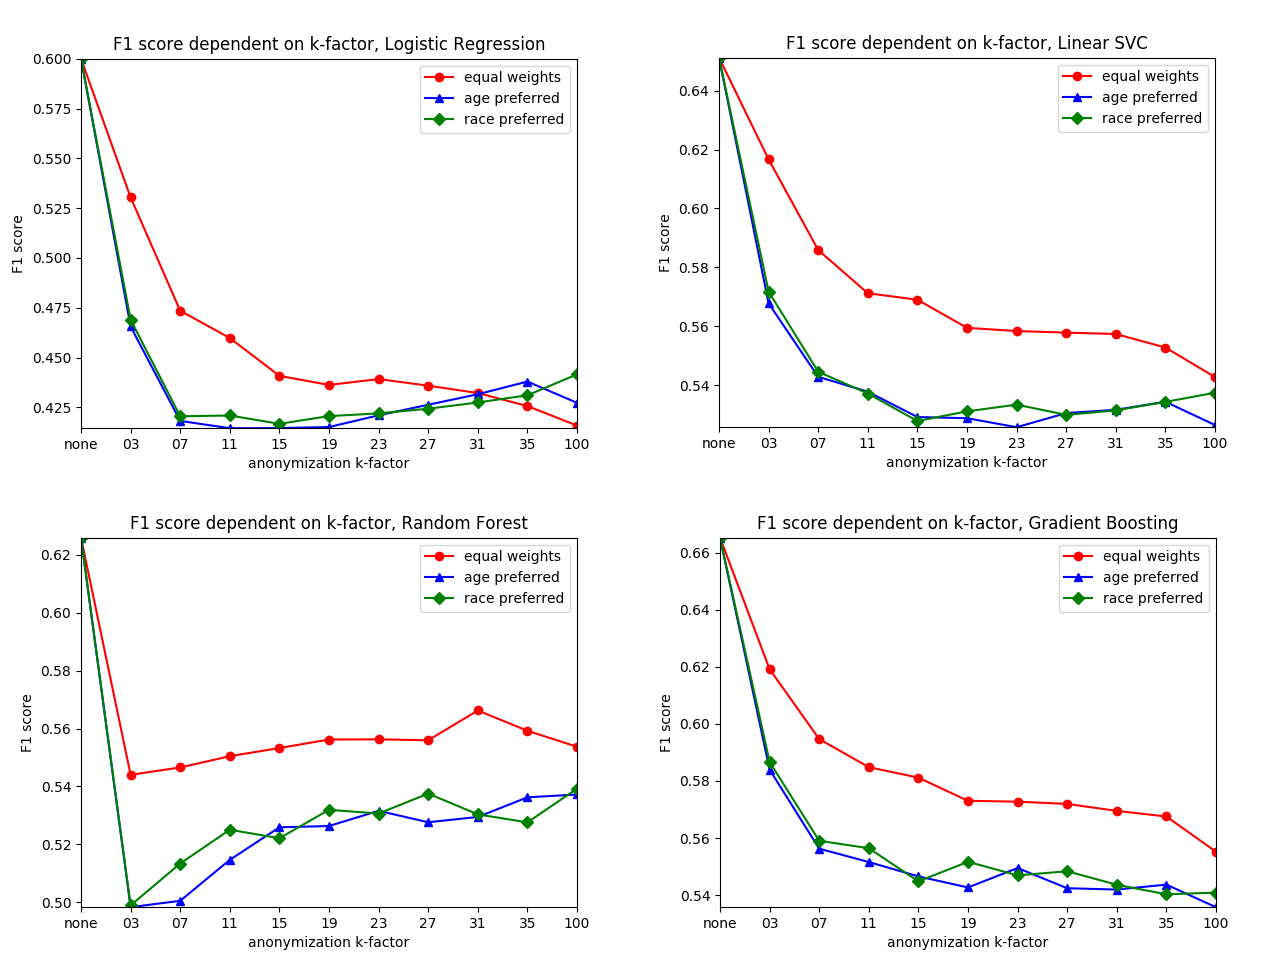
\includegraphics[width=1\textwidth]{figures/anonymization/adults_education_num/anon_education_combined}
	\caption{Multi-class classification on target \textit{education-num} on the adult dataset under several degrees of k-anonymization.}
	\label{fig:results_anonymization_education_num}
\end{figure}

Classifier performance on target \textit{marital-status} displayed the same basic behavior as above, including the mysterious conduct of the Random Forest in case of our age- and race-vectors. Moreover, the classification results are generally better than for \textit{education-num}, which is probably caused by our somewhat arbitrary clustering of education levels during pre-processing. All in all, the pure anonymization-related results were almost in line with our expectations; in addition, our previous assessment that implementation of the 'right-to-be-forgotten' for individual users is preferable to wholesale anonymization, has not changed for the multi-class case.


\begin{figure}[!h]
	\centering
	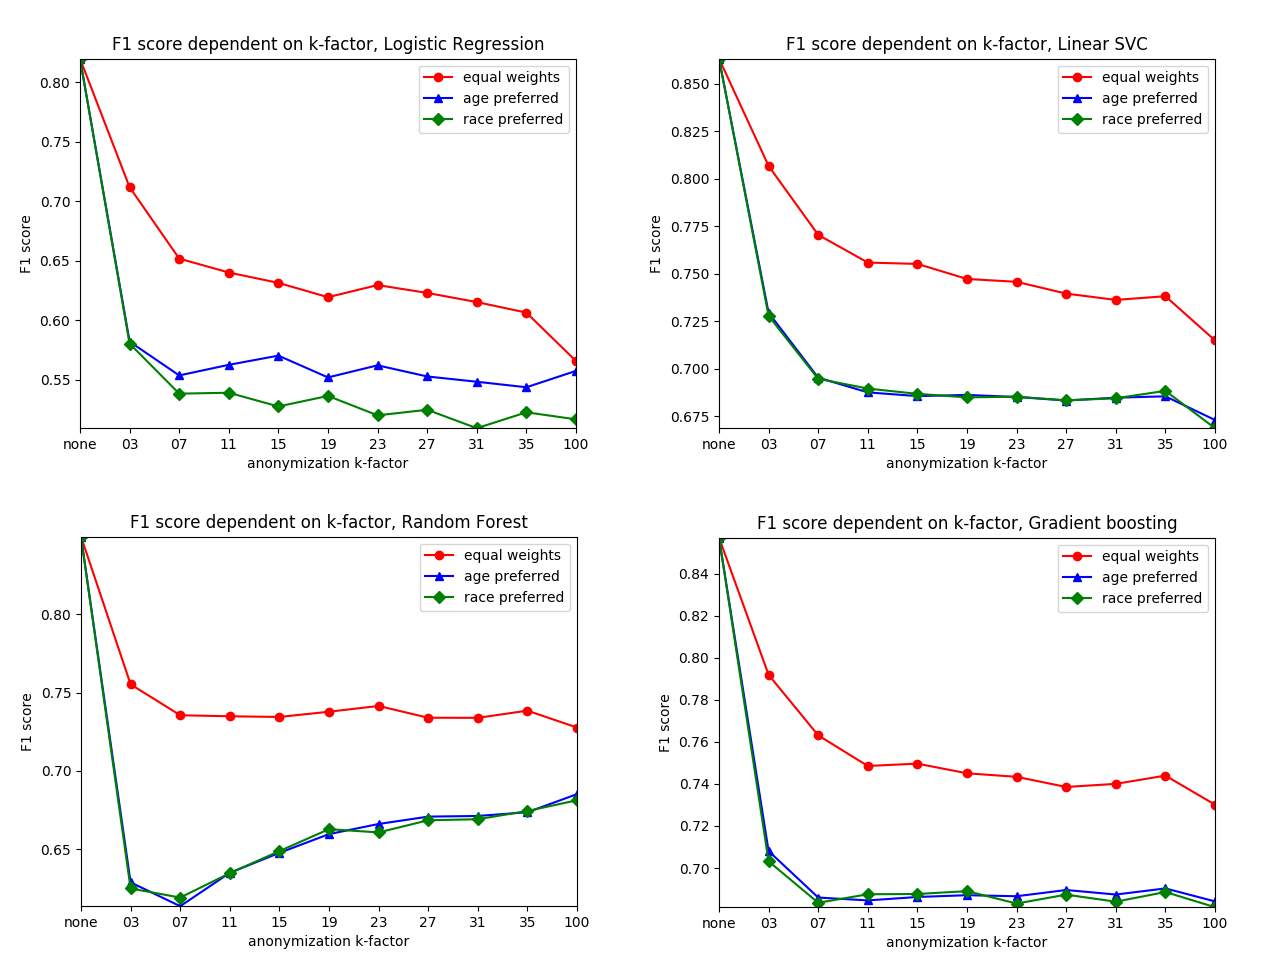
\includegraphics[width=1\textwidth]{figures/anonymization/adults_marital_status/anon_marital_combined}
	\caption{Multi-class classification on target \textit{marital-status} on the adult dataset under several degrees of k-anonymization.}
	\label{fig:results_anonymization_marital_status}
\end{figure}




\subsection{"Outliers" removed}
\label{ssect:outliers_removed}

One question we didn't tackle in our previous work was the one of outlier removal; this is relevant due to the fact that e.g. people showing abnormal behavior could be supposed to exercise their 'right-to-be-forgotten' more frequently, especially in a social network scenario. For our experiments we chose the original adult dataset's income target, especially since we could thus directly compare the results with those of our previous work \cite{malle2016right}. We used scikit-learn's Isolation-Forest classifier to identify outliers according to a given \textit{contamination} level and performed an initial round of removing outliers in a range of $0.5\% - 5\%$. Since ML performance decreased only marginally under those settings and we thus assumed that the dataset had been curated in such a way as to exclude significant outliers, we pivoted to a much broader investigation of examining classifier performance on a dataset with increasingly eviscerating variance. Thus we repeated the same procedure for "outlier" levels of $5\% - 95\%$, gradually diminishing the dataset's size from over 30k to about 1.5k data points. In order to account for that dramatic reduction, we compared classifier behavior with a control instance of the adult dataset with the same levels of truncation, but under random deletion of data points, thus not targeting variance in the control set. 

The results are shown in Figure~\ref{fig:results_outliers_removed} and exhibit similar behavior to the removal of most-significant attribute values in our previous work: While performance only decreases slightly for deletion levels under $55\%$, we see a dramatic drop over the second half of the range. The obvious explanation for this behavior lie in the fact that more homogeneous clusters of data make it harder for any algorithm to construct a decision boundary - though it is noteworthy that this applies to all 4 classifiers the same despite their fundamentally different approaches. Lastly, the comparison set shows no significant increase / decrease of performance over the whole range of data deletion, supporting our conclusion that decreasing data set size was not the dominating influence for the observed algorithmic behavior.


\begin{figure}[!h]
	\centering
	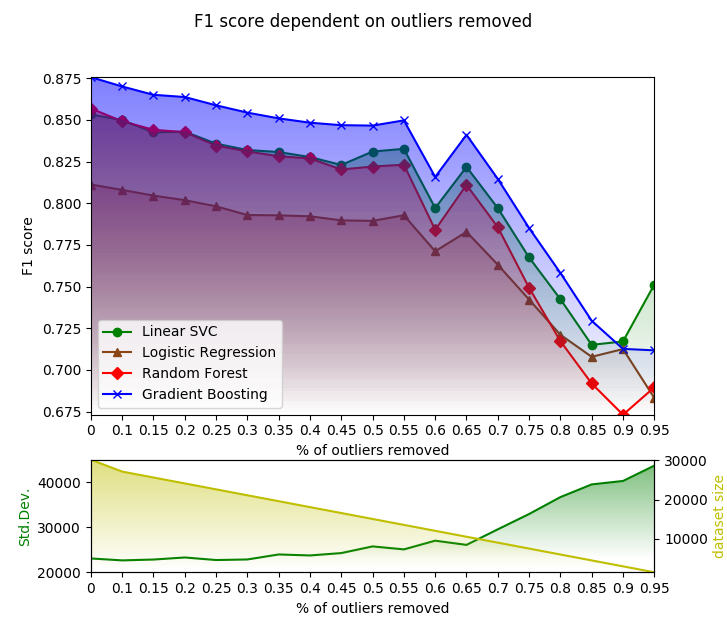
\includegraphics[width=0.49\textwidth]{figures/outliers/outliers_removed_all_algos_std_blur_bright}
	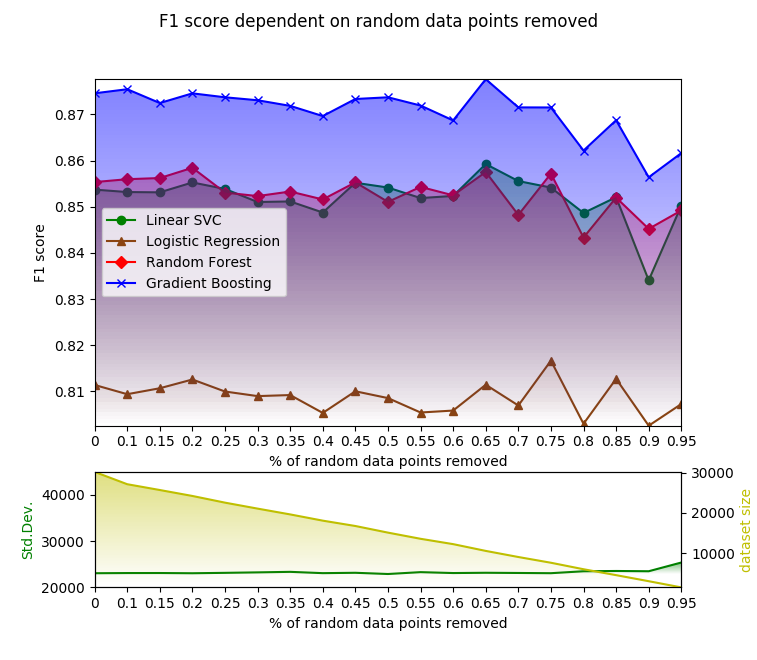
\includegraphics[width=0.49\textwidth]{figures/outliers/randomly_removed_points_all_algos_std_blur_bright}
	\caption{Binary classification on target income based on a dataset with different degrees of outliers removed (= variance loss) vs. the same degree of data randomly deleted.}
	\label{fig:results_outliers_removed}
\end{figure}



\subsection{Anonymization on Outliers removed}
\label{ssect:anon_outliers_removed}

One problem with outliers during anonymization is that it forces the algorithm to over-generalize attribute values; this can either happen towards the end-stages of a greedy-clustering procedure like SaNGreeA (in which case the damage might be limited to the outliers themselves), but could also influence a full-domain generalizing algorithm during determination of a whole column's suitable generalization level (in which case the whole dataset would suffer significantly higher information loss). This fact in combination with our previously described results based on outlier removal gave rise to an interesting possibility: what if we \textit{combined} outlier removal with anonymization? On the one hand classifier performance degrades with loss of variance, but for the very same reason information loss during anonymization might be limited to much more sufferable levels.

This led to our last round of experiments in which we took the adult dataset with 30\% outliers removed and conducted k-anonymization as described in the respective earlier section (for time- and comparison reasons only on marital-status), the results of which can be seen in Figure~\ref{fig:results_anonymization_outliers_marital_status}. We were astonished to observe that - for the most part - classifiers performed better under this setting than under anonymization alone. For logistic regression, although age \& race vectors performed worse then their anonymized-only counterparts, performance for equal weights was better for $k<11$. With Random Forest, all vectors performed better than their anonymization-only counterparts, with $k=3$ only 2\% below original performance. With Linear SVC, age \& race performed worse at the beginning only to recover with increasing performance towards $k=100$, whereas the equal vector behaved about equal to it's non-outlier-removed opposite. Finally, Gradient Boosting in this setting outperforms it's anonymization-only competitor in all settings with it's $k=3$ equal weight vector performance lying within only half a percentage point of the performance on the original, un-anonymized dataset.

As a side-note, we observe that under these settings, SVC starts to mimic Random Forest's behavior of an initial collapse in performance for the age- and range-vectors with a subsequent recovery towards higher levels of $k$. We do not yet have an adequate explanation for this and will investigate deeper in our future efforts. 

\begin{figure}[!h]
	\centering
	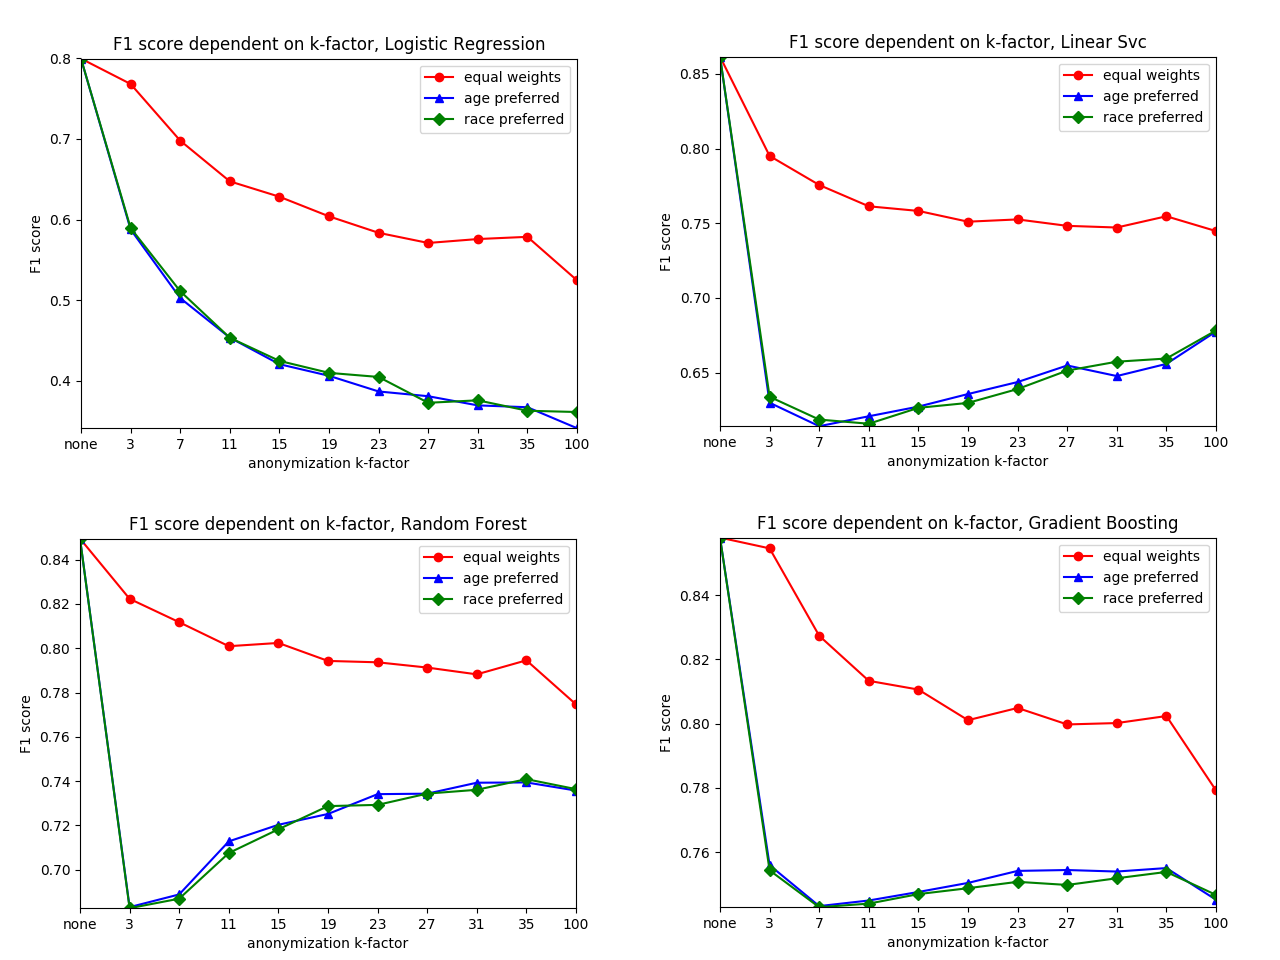
\includegraphics[width=1\textwidth]{figures/anon_outliers/anon_outliers_marital_combined}
	\caption{Multi-class classification on target marital status based on a dataset with 30\% outliers removed AND under different degrees of k-anonymization.}
	\label{fig:results_anonymization_outliers_marital_status}
\end{figure}

Those amazing results raise a few burning questions: 1) Can we repeat that performance on real-world data? 2) Could we combine this technique with interactive Machine Learning / Anonymization which yield better weight vectors? 3) Do those advantages only hold for a toy algorithm or will they persist under more sophisticated Anonymization pipelines? 4) Can we further enhance those results by mixing synthetic data into the dataset? 5) Will better feature engineering compensate for our original drop in performance and thus moot our insight? and 6) can we apply this conclusion to other data structures like social networks? These points shall now briefly be discussed before concluding the paper.


% ==================================
%			OPEN PROBLEMS
% ==================================
\section{Open problems / Future challenges}
\label{sect:op_fc}

\begin{enumerate}
	\item \textbf{Real world data}. Despite the convenient availability of well-curated datasets with many thousands of data rows, actual industry datasets are usually orders of magnitudes larger. This has consequences for their internal data topology and thus the performance of ML algorithms; e.g. \cite{brain1999effect} observe that variance error can be expected to decrease as training set size increases (though this might have nothing to do with variance in the dataset itself).
	
	\item \textbf{Interactive machine learning}. We have demonstrated experiments with different weight vectors in our approach regarding anonymization. However, data utility is highly subjective w.r.t. the specific area of application; therefore choosing the importance of attributes with regard to the particular environment is best done by a human. The problem of (k-)anonymization thus lends itself to interactive Machine Learning (iML) with a human-in-the-loop approach \cite{Holzinger:2016:iML}, \cite{Kieseberg:2016:Doctor-in-the-Loop}, \cite{iMLExperiment}. We have implemented software for iML Anonymization and are currently collecting test results which will soon be ready for publication.
	
	\item \textbf{Real world algorithms}. While we only anonymizing our datasets via simple k-anonymization through greedy clustering, there are much more sophisticated algorithms available, capable of fine-tuning generalization levels to the specific data topology of an input set in order to minimize information loss. It remains to be seen if such algorithms can still profit from removal of outliers as a pre-processing step.
	
	\item \textbf{Synthetic datasets}. In recent years it has become common to augment (small) datasets via synthetically generated, additional data-points \cite{wong2016understanding}. By controlling the data generation process, one would be able to also control variance-injection into a dataset. Therefore, instead of outlier-removal, one could enrich a dataset by introducing lower-variance data points before anonymization.
	
	\item \textbf{Better feature engineering}. For our experiments, we considered practically all columns of the adult dataset, although some exhibited much higher variance than others. It is therefore conceivable that by careful feature engineering the basis for anonymization could be sufficiently improved, rendering outlier-removal unnecessary.

	\item \textbf{Graph structure anonymization}. This includes questions of measuring structural outliers in a graph (maybe via centrality- or component-based analysis?) as well as outlier removal (do they have to be deleted or will randomly adding edges to such nodes suffice?). Our team is currently devising experiments in this direction, but our efforts are still in the early stages.
\end{enumerate}


% ==================================
%			CONCLUSION
% ==================================
\section{Conclusion}
\label{sect:conclusion}

In this paper we continued our initial experiments on the effects of anonymization and perturbation of knowledge bases on classifier performance and expanded our efforts to multi-class classification, outlier-removal as well as a combined outlier/anonymization approach. Our results show that selective deletion of significant attribute values is preferable to general anonymization, insofar a dataset's topology allows for such conduct. We have furthermore seen that reducing variance in a dataset prevents algorithms of different breeds alike from finding efficient discriminators between classes, leading to a significant degradation of machine learning performance. Finally, we were astonished to observe that combining outlier-removal with anonymization can - under circumstances - yield almost as good a performance as classification on the original, un-anonymized dataset itself. We believe that this insight, in combination with work on interactive Anonymization we are currently conducting, state-of-the art anonymization techniques (we were using a rather simple algorithm for this paper), as well as the introduction of synthetic data, will enable us to soon propose competitive Machine Learning pipelines for real-world usage to counterbalance any regulatory disadvantage European companies are currently facing on the marketplace.

\clearpage
\newpage

\bibliographystyle{plain}
\bibliography{references}

\end{document}
